\section{Padrões e Normas}
\subsection{ITIL}

A ITIL define serviço como um meio intangível de entregar valor aos clientes,
facilitando resultados sem ter que assumir custos e riscos extras.E a ITIL mapeia
todo o ciclo de vida dos serviços através de 5 pilares:
\begin{itemize}[noitemsep]
  \item Estratégia do Serviço
  \item Desenho de Serviço
  \item Transição de Serviço
  \item Operação do Serviço
  \item Melhoria Continuada
\end{itemize}

Estratégia do Serviço (“Service Strategy”): É aqui que são tomadas as deciões estratégicas relacionadas aos serviços que vão ser desenvolvidos. Serviços que ajudam na identificação de requisitos e outras necessidades que ajudam a alcançar os objetivos do negócio.

Desenho de Serviço (“Service Design”): Basicamente desenha o que a estratégia decidiu, tendo em mente os fatores de utilidade e garantia, tomando por base as características esperadas para os serviços e culminando na elaboração e descrição de especificações dos serviços.

Transição de Serviço (“Service Transition”): Tem por foco o gerenciamento de mudanças, prevendo para tal fim a condução de ações voltadas à implantação de serviços. Move os serviços para o ambiente de produção. Os serviços são desenvolvidos, testados e liberados de forma controlada.

Operação do Serviço (“Service Operation”): Aqui estão os processos do dia-a-dia, que mantém os serviços funcionando assegurando que seus objetivos sejam alcançados, baseando-se para isto, em acordos de níveis de serviços (SLAs, sigla do inglês “Service-level Agreements”).

Melhoria Contínua do Serviço (“Continual Service Improvement”): Busca constante pela evolução dos serviços, aplicando para isto conceitos oriundos de técnicas como o ciclo PDCA (sigla do inglês “Plan-Do-Check-Act”).

\cite{itsmfservice}Esses pilares, se destrinchados, nos fornecem um total de 26 processos e 4 funções, aprofundando o conceito de como estruturar um serviço de acordo com áreas, fases do ciclo de vida e funções.



As práticas de ITIL procuram fornecer o suporte necessário para que tais serviços estejam em sintonia com as necessidades do negócio.Dentre os benefícios que podem ser obtidos a parte da utilização das técnicas que compõem ITIL, pode-se destacar:


\begin{itemize}[noitemsep]
	\item Melhorias na satisfação dos clientes/áreas dependentes de um ou mais serviços;
	\item Maior eficiência operacional;
	\item Redução nos custos e nos esforços desprendidos pela área de TI cumprimento de uma ampla gama de atividades;
\end{itemize}

Foi escolhida a utilização do ITIL versão 3 (Adams, et al., 2009), denominada
V3, por ser um framework aberto e bastante aceito na comunidade. Esta versão é
composta por cinco livros, onde cada um deles está relacionado a um estágio do
ciclo de vida do serviço. Na realização deste trabalho houve o foco apenas no
estágio que trata do serviço, isto é, o “Service Operation”;\\

\subsubsection{Operação de Serviço}
Operação de serviço é o mais relevante para suporte ao usuário
O propósito da Operação de Serviços é coordenar e realizar as atividades e processos q
requeridos para entregar e gerenciar os serviços em níveis acordados com usuários e
clientes(Livro)
Enquanto as fases anteriores englobam processos mais estraté-
gicos e táticos, a Operação de Serviço representa o dia a dia do pessoal de TI, com processos e
funções operacionais

\paragraph{Processos}
\begin{itemize}[noitemsep]
	\item Gerenciamento de Evento
	\item Gerenciamento de incidente
	\item Gerenciamento de Problema
	\item Gerenciamento de Acesso
	\item Execução de Requisição
\end{itemize}

\subparagraph{Gerenciamento de eventos}
Um evento pode ser descrito como qualquer ocorrência detectável ou discernível que q
seja significativa para a gestão da infraestrutura de TI ou para a entrega do serviço de TI (Livro)
Eventos são notificações criadas por um serviço de TI, item de configuração ou ferramenta
de monitoração.\\ A Operação de Serviço eficiente depende do conhecimento da situação
da infraestrutura e da detecção de qualquer desvio da operação normal ou esperada.


\subparagraph{Gerenciamento de incidentes}
O processo de Gerenciamento de Incidente procura restaurar os serviços o mais rápido
possível com o mínimo de interrupção, minimizando os impactos negativos nas áreas de negócio

Possui processos mais reativos, pois entraram em atuação a partir dos incidentes
levantados por usuários, importante considerar também que as informações dos
incidentes levantadas neste processo serão de grande importância para o processo
de Gerenciamento de Problema.
\\
\begin{figure}[!h]
\caption{Gerenciamento de incidentes retirado do ITIL v3 Fundation}
\centering % para centralizarmos a figura
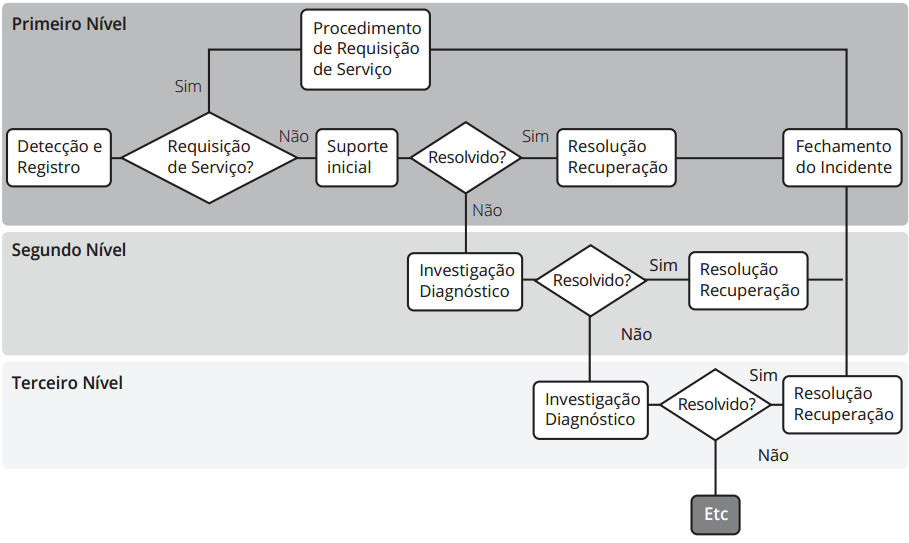
\includegraphics[width=15cm]{itil_images/gerenciamento_de_incidentes.png}
\label{figura:Gerenciamento de incidentes retirado do ITIL v3 Fundation}
\end{figure}

\subparagraph*{Conceitos}
\begin{itemize}[noitemsep]
	\item {\bfseries Prazos para execução e escalonamento (Timescales)} \\
		Prazos de execução precisam ser acordados para todos os estágios de tratamento ao inci-
		dente (que irão diferir de acordo com a prioridade do incidente)

	\item {\bfseries Modelos de Incidente (Incident Models) } \\
		Um modelo de incidente é uma forma de pré-definir os passos que devem ser seguidos
		para manusear um incidente, de maneira acordada. Define os passos a serem executados, a
		ordem cronológica dos passos, responsabilidades, tempos de execução, procedimentos de
		escalonamento e geração de evidências.

\end{itemize}


\subparagraph{Gerenciamento de Problema}
Uma forma de reduzir a quantidade de incidentes é evitando a sua recorrência. Através q
do processo de Gerenciamento de Problema, os problemas com causas não identificadas
serão analisados e corrigidos para que não voltem a acontecer.
É importante que o processo de Gerenciamento de Problema venha acompanhado do
Gerenciamento de Mudança, fazendo com que a correção dos erros seja previamente
analisada em relação aos riscos. Muitas vezes a correção de um erro acaba gerando mais
incidentes e criando impacto para os usuários.

Este processo tem como missão minimizar a interrupção nos serviços de TI através da orga-
nização dos recursos para solucionar problemas de acordo com as necessidades de negócio,
prevenindo a recorrência dos mesmos e registrando informações que melhorem a maneira
pela qual a organização de TI trata os problemas, resultando em níveis mais altos de disponibilidade e produtividade.

\begin{figure}[!h]
\caption{Gerenciamento de problema retirado do ITIL v3 Fundation}
\centering % para centralizarmos a figura
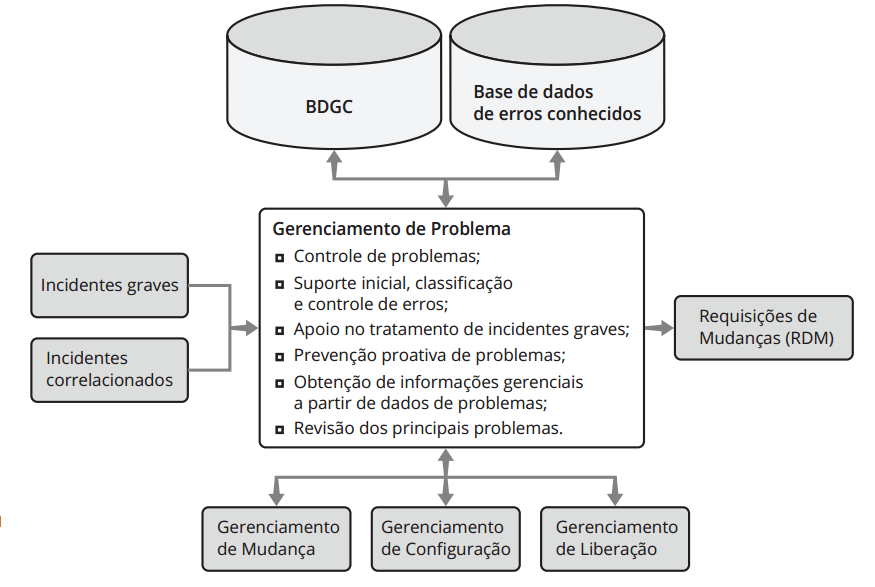
\includegraphics[width=15cm]{itil_images/gerenciamento_de_problema.png}
\label{figura:Gerenciamento de problemas retirado do ITIL v3 Fundation}
\end{figure}

\subparagraph*{Conceitos}
\begin{itemize}[noitemsep]
	\item {\bfseries Modelos de Problemas (Problem Models)} \\
		Muitos problemas são únicos e devem receber tratamento individual. Porém, alguns incidentes 				podem ocorrer novamente por causa de problemas adormecidos ou camuflados.
	\item {\bfseries Base de Dados de Erros Conhecidos (Know Error Database) } \\
		O propósito dessa base de dados é permitir o armazenamento de conhecimentos prévios a
	respeito de incidentes e problemas (e como eles foram superados), possibilitando assim o
	diagnóstico e resolução rápidos. O registro de erros conhecidos deve conter todos os detalhes da 		falha ocorrida e seus respectivos sintomas, juntamente com detalhes de qualquer solução de contorno 		que venha a ser realizada para solucionar incidentes ou problemas.
\end{itemize}





\subparagraph{Gerenciamento de acesso}

Este processo ajuda a organização a manter a confidencialidade das suas informações de
forma mais efetiva. O Gerenciamento da Segurança da Informação define as políticas de
segurança, enquanto o Gerenciamento de Acesso executa o que foi definido a partir destas
políticas, sendo assim uma parte operacional da segurança da informação.
Concede ao usuário o direito de usar um serviço, mas nega o acesso a usuários não autorizados.

\begin{figure}[!h]
\caption{Gerenciamento de acesso retirado do ITIL v3 Fundation}
\centering % para centralizarmos a figura
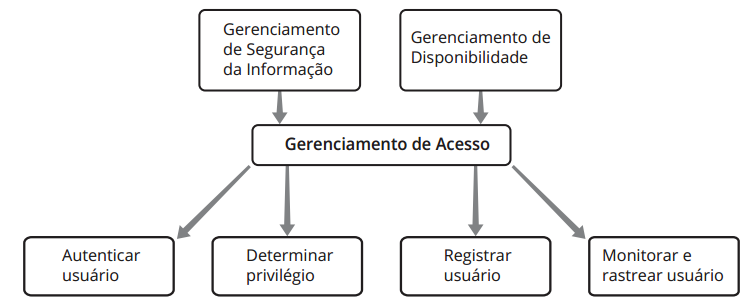
\includegraphics[width=15cm]{itil_images/gerenciamento_de_acesso.png}
\label{figura:Gerenciamento de acesso retirado do ITIL v3 Fundation}
\end{figure}

\subparagraph*{Conceitos}
Gerenciamento de Acesso está fundamentado nos conceitos listados abaixo
\begin{itemize}[noitemsep]
	\item {\bfseries Acesso (Access) }
		Refere-se ao nível e extensão da funcionalidade de um serviço ou dado permitido a um usuário.
	\item {\bfseries Identidade (Identity) }
		Refere-se à informação sobre o usuário, que o distingue dos demais e demonstra sua situação 				dentro da organização.
	\item {\bfseries  Direitos ou Privilégios (Rights) }
		Referem-se à regulamentação definida, que determina o acesso a ser oferecido ao usuário
		para um serviço ou grupos de serviços.
\end{itemize}





\subparagraph{Execução de requisição}
O termo Execução de Requisição é usado como uma descrição genérica para muitos tipos de demandas colocadas sobre a área de TI por seus usuários (Requisição de Serviço).
Muitas delas são na verdade pequenas mudanças de baixo risco, ocorrendo com frequência.



\begin{figure}[!h]
\caption{Execução de requisição do ITIL v3 Fundation}
\centering % para centralizarmos a figura
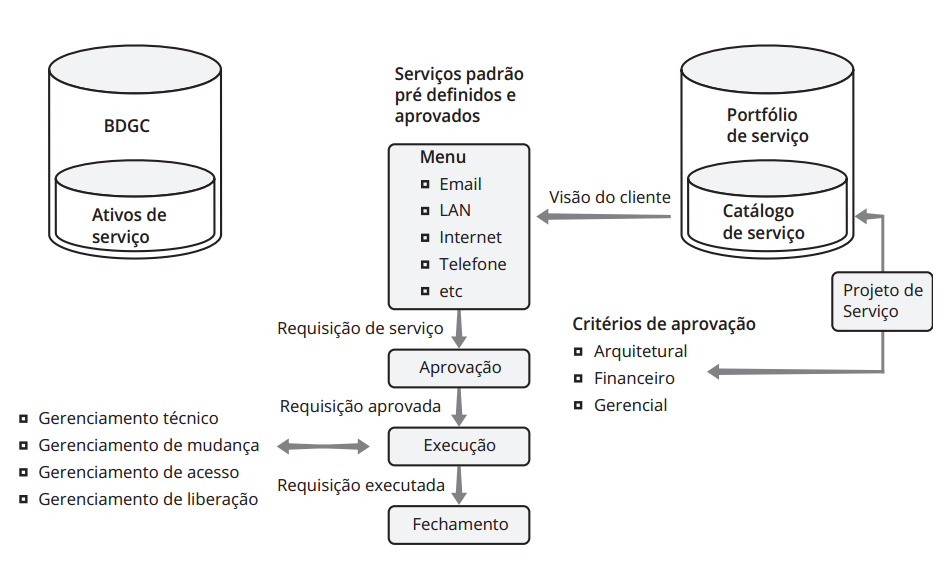
\includegraphics[width=15cm]{itil_images/execucao_de_requisicao.png}
\label{figura:Execução de requisiçao retirado do ITIL v3 Fundation}
\end{figure}




\subparagraph*{Conceitos}
Solicitações de serviço ocorrem frequentemente e requerem seu atendimento através de
uma maneira consistente, de forma a atender os níveis de servidos acordados. Para dar
assistência a essas solicitações, muitas organizações criam Modelos de Requisições (Request
Models) pré-definidos, os quais tipicamente incluem alguma forma de pré-aprovação por
parte do processo de Gerenciamento de Mudança.
